% Define a section
\section{Názov kapitoly}
% Use an acronym
Prvé použitie skratky \gls{UML} zobrazí definíciu. Každé ďalšie použitie zobrazí \gls{UML}.\\
Prvé použitie skratky \gls{OCL} zobrazí definíciu. Každé ďalšie použitie zobrazí \gls{OCL}.\\
Prvé použitie skratky \gls{BPMN} zobrazí definíciu. Každé ďalšie použitie zobrazí \gls{BPMN}.

% Define a subsection
\subsection{Názov podkapitoly}
Lorem ipsum dolor sit amet, consectetur adipiscing elit. Integer eu lacus leo. Nulla egestas purus non dignissim tincidunt.
% Add a list
\begin{itemize}
    \item Položka zoznamu
    \item Položka zoznamu
\end{itemize}
\hfill
\begin{enumerate}
    \item Položka číslovaného zoznamu
    \item Položka číslovaného zoznamu
\end{enumerate}

% Add a figure
\begin{figure}[h]
    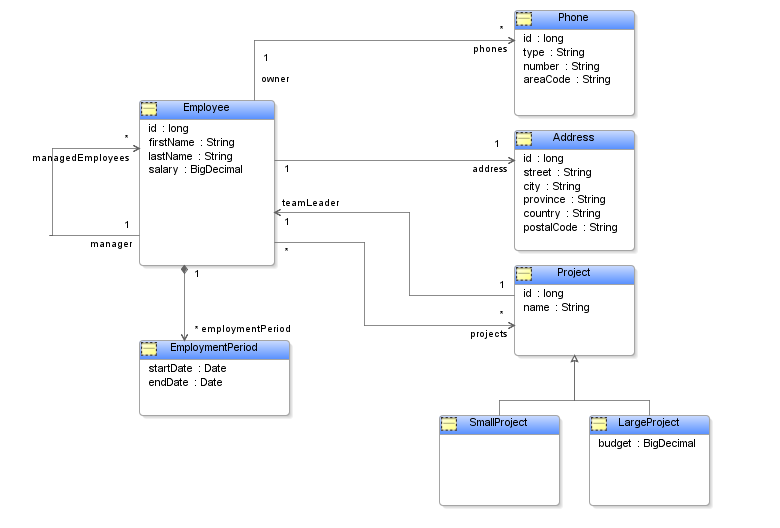
\includegraphics{examples/images/employee-model.png}
    \caption{UML diagram zamestnanca}
    \label{fig:example1}
\end{figure}

% Add citations
\newpage
\noindent
Odkazy na použitú literatúru \parencite{luptak2016thesis} alebo \textcite{borgman2003from}.\footnote{V prípade nejasností alebo pre lepšie pochopenie niektorých pojmov jazyka boli ďalej využívané aj zdroje \parencite{lynch2005where} a \parencite{luptak2016thesis}}
\\Pre citácie používajte normu STN ISO 690, môžete citovať aj v tvare [1], [2],… vtedy v zozname literatúry neuvádzate zdroje abecedne, ale ich uvádzate podľa poradia výskytu v texte. 

% Define a subsubsection
\subsection{Môžete vložiť novú podkapitolu}
\subsubsection{Taktiež aj na úrovni 3}

% Add a table
\begin{table}[!h]
    \centering
    \caption{Názov tabuľky}
    {\color{red} \textbf{Pánsky dres - strih Classic}}\\
    \vspace{1em}
    \rowcolors{2}{white}{gray!30}  
    \begin{tabular}{cccc}  
        \textbf{dres - veľkosť} & \textbf{obvod hrudník} & \textbf{obvod pás (guma)} & \textbf{dĺžka zadného dielu (od krku)} \\
        XS & 96 & 72-80 & 69 \\
        S & 100 & 76-84 & 70 \\
        M & 104 & 80-80 & 71 \\
        L & 108 & 84-96 & 72 \\
        XL & 112 & 88-100 & 73 \\
        XXL & 116 & 92-104 & 75 \\
        XXXL & 120 & 96-108 & 77 \\
    \end{tabular}
    \label{tab:example}
\end{table}

% Add a code block
\begin{lstlisting}[language=Python, caption={Príklad kódu v Pythone}, label={lst:python-example}]    
def hello_world():
    print("Hello, world!")
        
# Example class
class Person:
    def __init__(self, name):
        self.name = name
    
    def greet(self):
        return f"Hello, my name is {self.name}"

# Create instance
person = Person("Alfred")
print(person.greet())
\end{lstlisting}
